\appendix

\section{Implementation Details}
\label{app:implementation_details}

Training used distributed data parallelism on three NVIDIA GeForce RTX 5090 GPUs.
Table~\ref{tab:hardware_appendix} summarizes the hardware and runtime used for the final training run.

\begin{table}[htbp]
\centering
\small
\caption{Hardware and runtime used for the final training run.}
\label{tab:hardware_appendix}
\begin{adjustbox}{max width=\linewidth}
\begin{tabular}{p{0.38\linewidth} p{0.48\linewidth}}
\toprule
\textbf{Item} & \textbf{Value} \\
\midrule
Operating system & Linux 6.1.0-44-amd64 \\
CPU & 24 physical cores / 48 threads \\
System memory & 202 GB RAM \\
GPUs & 3 $\times$ NVIDIA GeForce RTX 5090 \\
GPU memory & 34 GB per GPU \\
Training parallelism & Distributed data parallel \\
Data-loader workers & 8 per process \\
Training runtime & 25.2 h for the complete training \\
\bottomrule
\end{tabular}
\end{adjustbox}
\end{table}

\section{MedNeXt-v2 Building Blocks}
\label{app:mednext_blocks}

Figure~\ref{fig:mednext_blocks} summarizes the core MedNeXt-v2 blocks used in LETT-NeXt.

\begin{figure}[htbp]
\centering
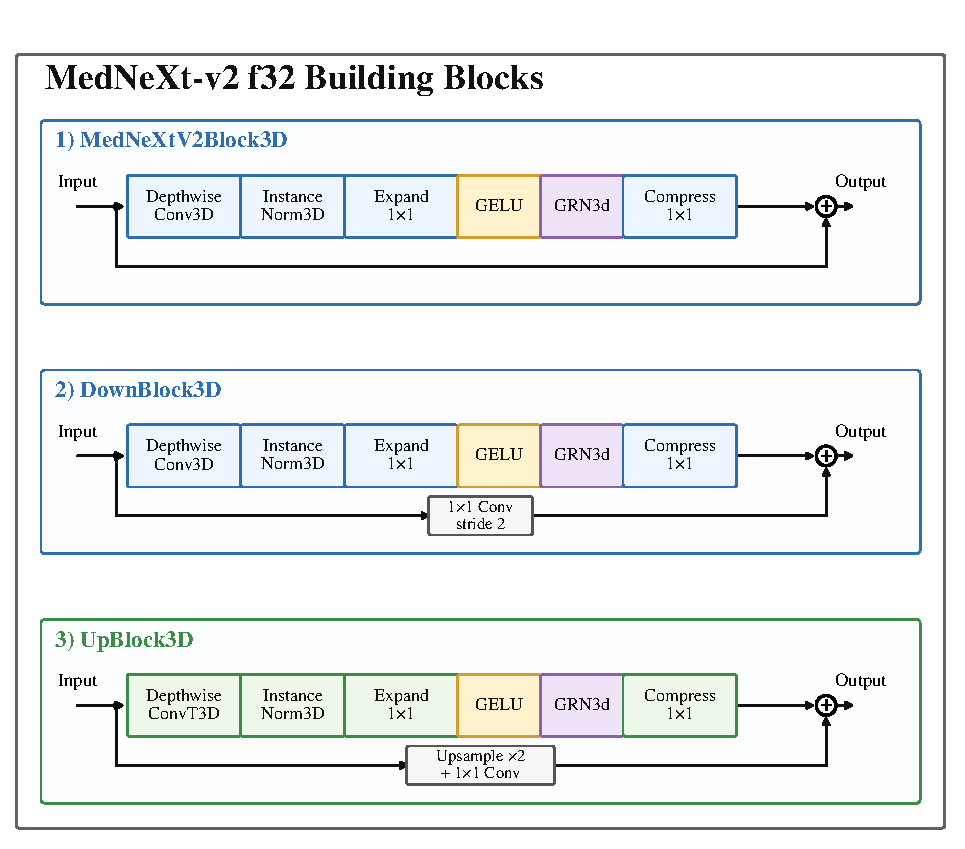
\includegraphics[
    width=\textwidth,
    trim={0 0 0 0.5cm},
    clip
]{images/mednext_blocks.pdf}
\caption{
Core MedNeXt-v2 building blocks used in LETT-NeXt.
The main block uses depthwise convolution, normalization, pointwise expansion and compression, GELU activation, global response normalization, and a residual connection.
The downsampling and upsampling blocks use residual projections to change spatial resolution.
}
\label{fig:mednext_blocks}
\end{figure}


\section{Controlled Ablation Details}
\label{app:controlled_ablation_details}

This appendix provides the shared protocol for the controlled ablations reported in Section~\ref{sec:ablation_studies}. The architecture ablation and auxiliary-head control used the same training data, crop geometry, prompt encoding, training schedule, validation set, and postprocessing unless otherwise stated. Paired improvements were computed from per-case validation-score differences on the 49-case validation set. Uncertainty was estimated using 95\% percentile bootstrap confidence intervals over validation cases.

For the prompt-removal diagnostic and AutoZoom reproduction, 95\% percentile confidence intervals used 10,000 paired bootstrap resamples of CT cases (seed 43). These intervals describe case-sampling uncertainty, not variation across training runs.

\subsection{Shared Training and Validation Setup}
\label{app:shared_ablation_setup}

All controlled ablation models were trained for 15 epochs with 625 steps per epoch and a global batch size of 8. This corresponds to 5,000 sampled crop presentations per epoch and 75,000 crop presentations in total. The crop size was \(64 \times 128 \times 128\) voxels and the target spacing was \(2.4 \times 1.0 \times 1.0\) mm, both given in \(z,y,x\) order.

The training data contained 25,112 records: 24,311 primary training records and 801 PanTS records. Validation was performed on the 49-case validation set. All models used the same three-channel input formulation defined in Section~\ref{sec:input_preprocessing}. The main output was a single binary lesion logit. The main lesion loss was Dice loss plus BCE loss with weights 1:2. Validation used prompt-component postprocessing, AutoZoom, threshold \(0.5\) unless otherwise stated, and cached dataset-statistics normalization.


\subsection{Architecture Ablation}
\label{app:architecture_ablation_details}

The architecture ablation compared five segmentation backbones under the shared setup described in Section~\ref{app:shared_ablation_setup}. The only intended experimental variable was the backbone architecture. Auxiliary anatomy supervision was disabled for all models in this ablation.

Table~\ref{tab:architecture_ablation_backbones} summarizes the backbones included in the comparison. All models used the same three-channel input formulation and binary lesion output, keeping the prompt representation fixed across backbones. The RECIST marker and endpoint maps were concatenated with the CT crop, so each backbone received the prompt as voxel-aligned image information.

\begin{table}[t]
\centering
\caption{
Overview of the backbones included in the architecture ablation.
}
\label{tab:architecture_ablation_backbones}
\footnotesize
\setlength{\tabcolsep}{4pt}
\begin{tabularx}{\textwidth}{@{}l@{\hspace{1.2em}}Xr@{}}
\toprule
\textbf{Model} & \textbf{Family} & \textbf{Params.} \\
\midrule
UNet base 
& 3D UNet 
& 1.19\,M \\

SegResNet 
& Residual CNN 
& 4.70\,M \\

SwinUNETR f24 
& Transformer--CNN hybrid 
& 15.70\,M \\

MedNeXt-v2 small 
& ConvNeXt-style 3D CNN 
& 1.28\,M \\

MedNeXt-v2 f32 
& ConvNeXt-style 3D CNN 
& 6.92\,M \\
\bottomrule
\end{tabularx}
\end{table}


\subsection{Auxiliary-Head Control}
\label{app:auxiliary_head_control}

The auxiliary-head control compared two MedNeXt-v2 small models under the shared setup described in Section~\ref{app:shared_ablation_setup}. The only intended experimental variable was whether the PanTS auxiliary anatomy--tumor head was enabled during training.

Table~\ref{tab:aux_head_threshold_sweep} reports the threshold sweep for the auxiliary-head control experiment. The auxiliary-head variant achieved a higher validation score at every swept threshold.

\begin{table}[t]
\centering
\caption{
Threshold sweep for the auxiliary-head control experiment.
Scores are reported on a \(0\)--\(100\) scale, and differences are reported in percentage points.
}
\label{tab:aux_head_threshold_sweep}
\begin{adjustbox}{max width=\linewidth}
\begin{tabular}{cccc}
\toprule
\textbf{Threshold} & \textbf{No aux score (\%)} & \textbf{Aux score (\%)} & \textbf{\(\Delta\) (pp)} \\
\midrule
0.35 & 66.13 & \textbf{67.09} & +0.96 \\
0.40 & 65.65 & 67.02 & +1.37 \\
0.45 & 65.41 & 66.78 & +1.37 \\
0.50 & 65.02 & 66.36 & +1.34 \\
0.55 & 64.84 & 65.79 & +0.95 \\
0.60 & 64.49 & 65.45 & +0.95 \\
0.65 & 63.96 & 64.77 & +0.81 \\
0.70 & 63.34 & 64.02 & +0.69 \\
0.75 & 62.58 & 63.32 & +0.74 \\
\bottomrule
\end{tabular}
\end{adjustbox}
\end{table}

The effect of auxiliary supervision was likely limited by its small share of the training data: PanTS contributed 801 of 25,112 training records, corresponding to 3.2\%. The auxiliary branch also learned a tumor signal on the 50-case PanTS auxiliary evaluation set, reaching an auxiliary tumor DSC of \(62.38\%\). These results should be interpreted as a matched single-run control rather than a multi-seed estimate.

\section{AutoZoom Triggered-Case Analysis}
\label{app:autozoom_cases}

AutoZoom was rerun on all 49 validation cases using the submitted settings. All first-pass predictions matched the saved fixed-crop results. Expansion triggered in three cases (Table~\ref{tab:autozoom_cases}). Case 0057 gained lesion coverage but added false positives. Case 0067 missed more lesion voxels and added false positives. Case 0095 missed more lesion voxels despite fewer false positives.

\begin{table}[htbp]
\centering
\small
\setlength{\tabcolsep}{4pt}
\caption{All triggered public-validation cases. Scores are averaged across target lesions within each case. Identifiers share the prefix CT\_Lesion\_FLARE23Ts\_. Each triggered prompt had label 1.}
\label{tab:autozoom_cases}
\begin{adjustbox}{max width=\linewidth}
\begin{tabular}{lrrr}
\toprule
\textbf{Case} & \textbf{Fixed score (\%)} & \textbf{AutoZoom score (\%)} & \textbf{$\Delta$ (pp)} \\
\midrule
0057 & 64.89 & 65.40 & +0.51 \\
0067 & 82.77 & 80.15 & -2.62 \\
0095 & 69.97 & 66.32 & -3.64 \\
\bottomrule
\end{tabular}
\end{adjustbox}
\end{table}


Figure~\ref{fig:autozoom_examples} shows examples where expansion helped or hurt segmentation. These examples come from training cases and are separate from the public-validation results in Table~\ref{tab:autozoom_cases}.

\begin{figure}[htbp]
    \centering
    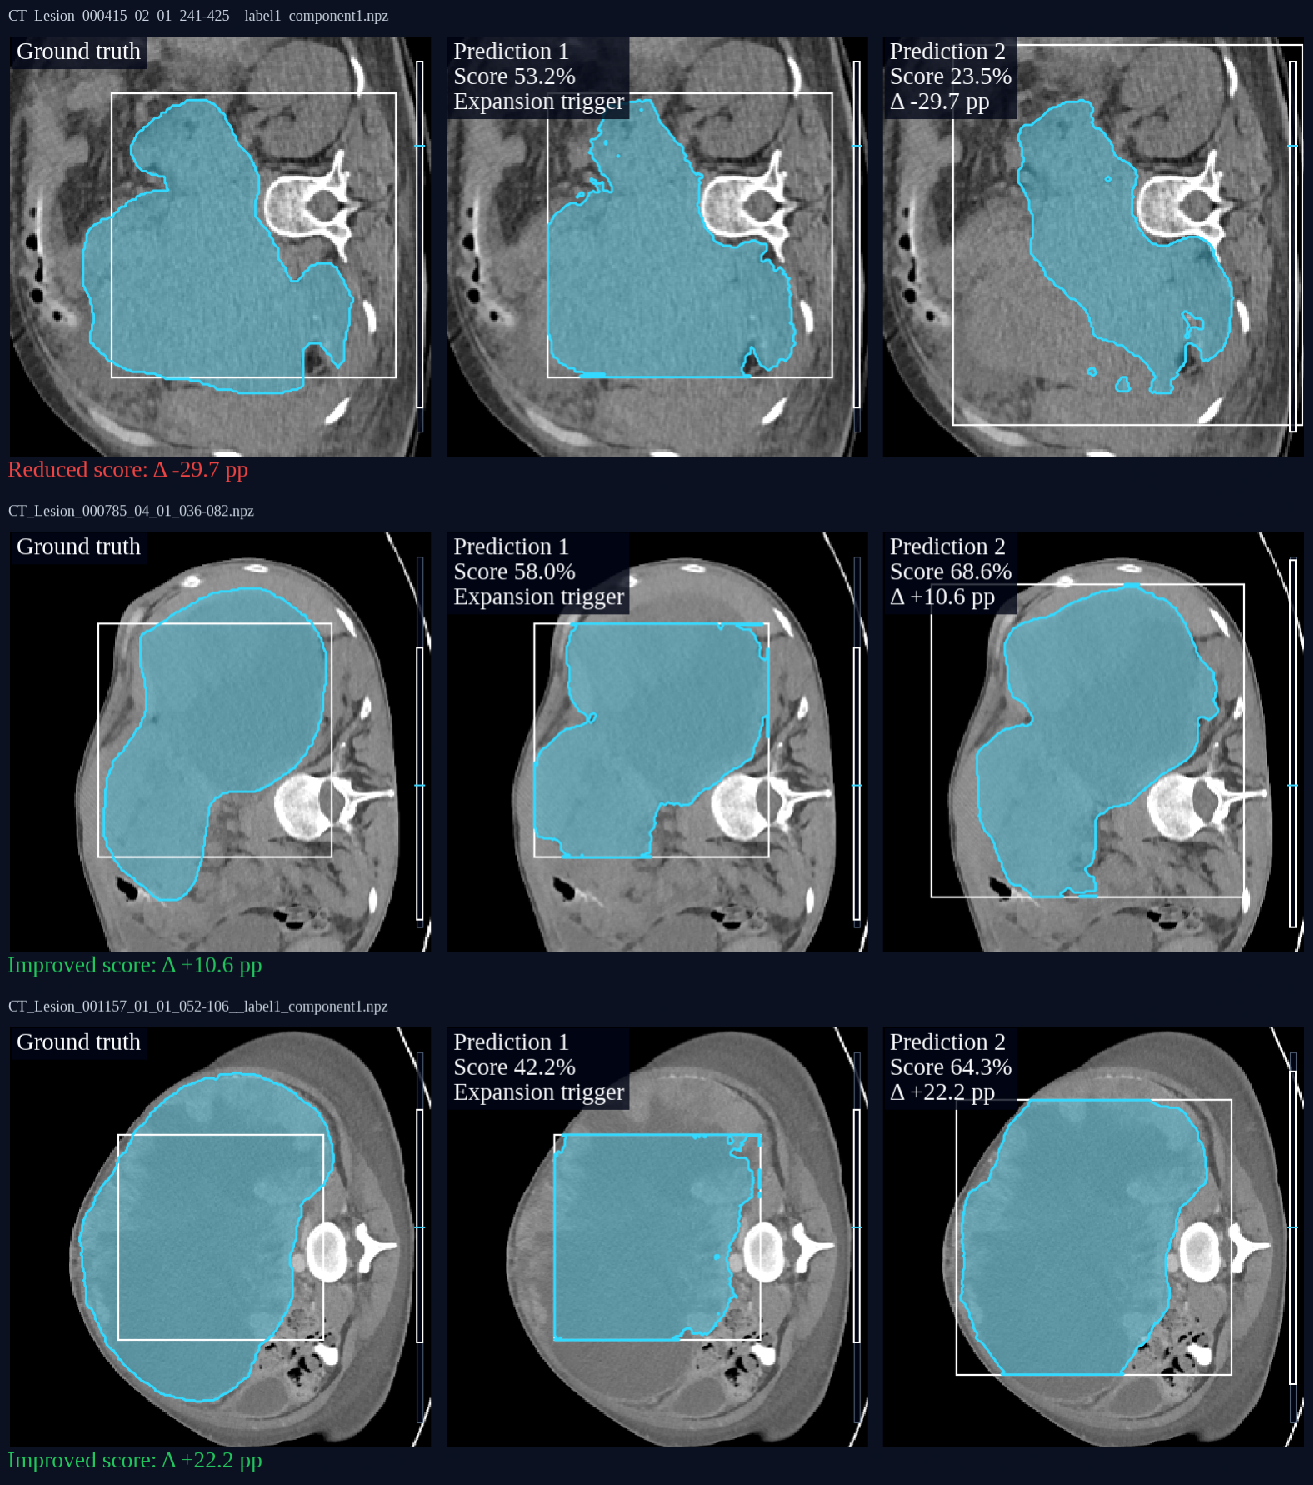
\includegraphics[width=0.85\linewidth,height=0.70\textheight,keepaspectratio]{images/task2_autozoom_xy_validation_selected_v2.pdf}
    \caption{Illustrative AutoZoom outcomes in training-set cases. Each row shows the reference, initial prediction, and prediction after expansion. White boxes indicate crop extent. The displayed scores describe the selected examples, not the three public-validation cases in Table~\ref{tab:autozoom_cases}.}
    \label{fig:autozoom_examples}
\end{figure}
